\documentclass{article}
\usepackage{graphicx} % Required for inserting images
\usepackage{gensymb}
\usepackage{caption}

\begin{document}

\section{Op Amp Overview}

The purpose of this section is to highlight the design of a voltage
amplIfier used to amplIfy the small voltage dIfference of a the k-thermocouple of $41\frac{{\mu}V}{C\degree}$ to a voltage dIfference of approximately $12.42\frac{mV}{C\degree}$. In the following subsections the circuit schematic and simulation of the OP07C operational amplIfier will be shown.

\subsection{Circuit Diagram}

The circuit schematic used to simulate and implement our Op-amp is shown below and follows the layout shown in the ELEC 291 project 1 lecture slides. The circuit diagram below was built and simulated in LTspice.
    \begin{figure}[h]
        \centering
        \includegraphics[width=0.5\linewidth]{Op07 Schreenshot.png}
        \caption{Voltage AmplIfier Circuit Diagram}
        \label{fig:Op-Amp}
    \end{figure}
\subsection{Circuit Simulation}
From the lecture slides it was shown that the gain of the voltage amplIfier is approximately $\frac{R1}{R2}$. When designing our voltage amplIfier we aimed to have a gain close to or above $10\frac{mV}{C\degree}$. To achieve this we performed a parameter sweep of the resistor R2 while holding t R1 constant. We chose to use large resistance values as smaller resistors were supposed to be allocated for any smaller scale functionality such as LEDs. To achieve the desired output voltage of 10mV or higher we found our gain must be at least $244\frac{V}{V}$. For the large resistor R1 we chose the largest value of $10M\ohm$. Then using the values of resistors provided in the project 1 kit a parameter sweep through resistor values 4.7k\ohm, 5.6k\ohm, 10k\ohm, 15k\ohm, 20k\ohm, 22k\ohm, 33k\ohm, 47k\ohm, 100k\ohm, and 470k\ohm\ was done on R2 to find the necessary value to get close to our output voltage requirements. The result of this parameter sweep is shown in the figure on the next page.
\newpage
 \begin{figure}[h]
        \centering
        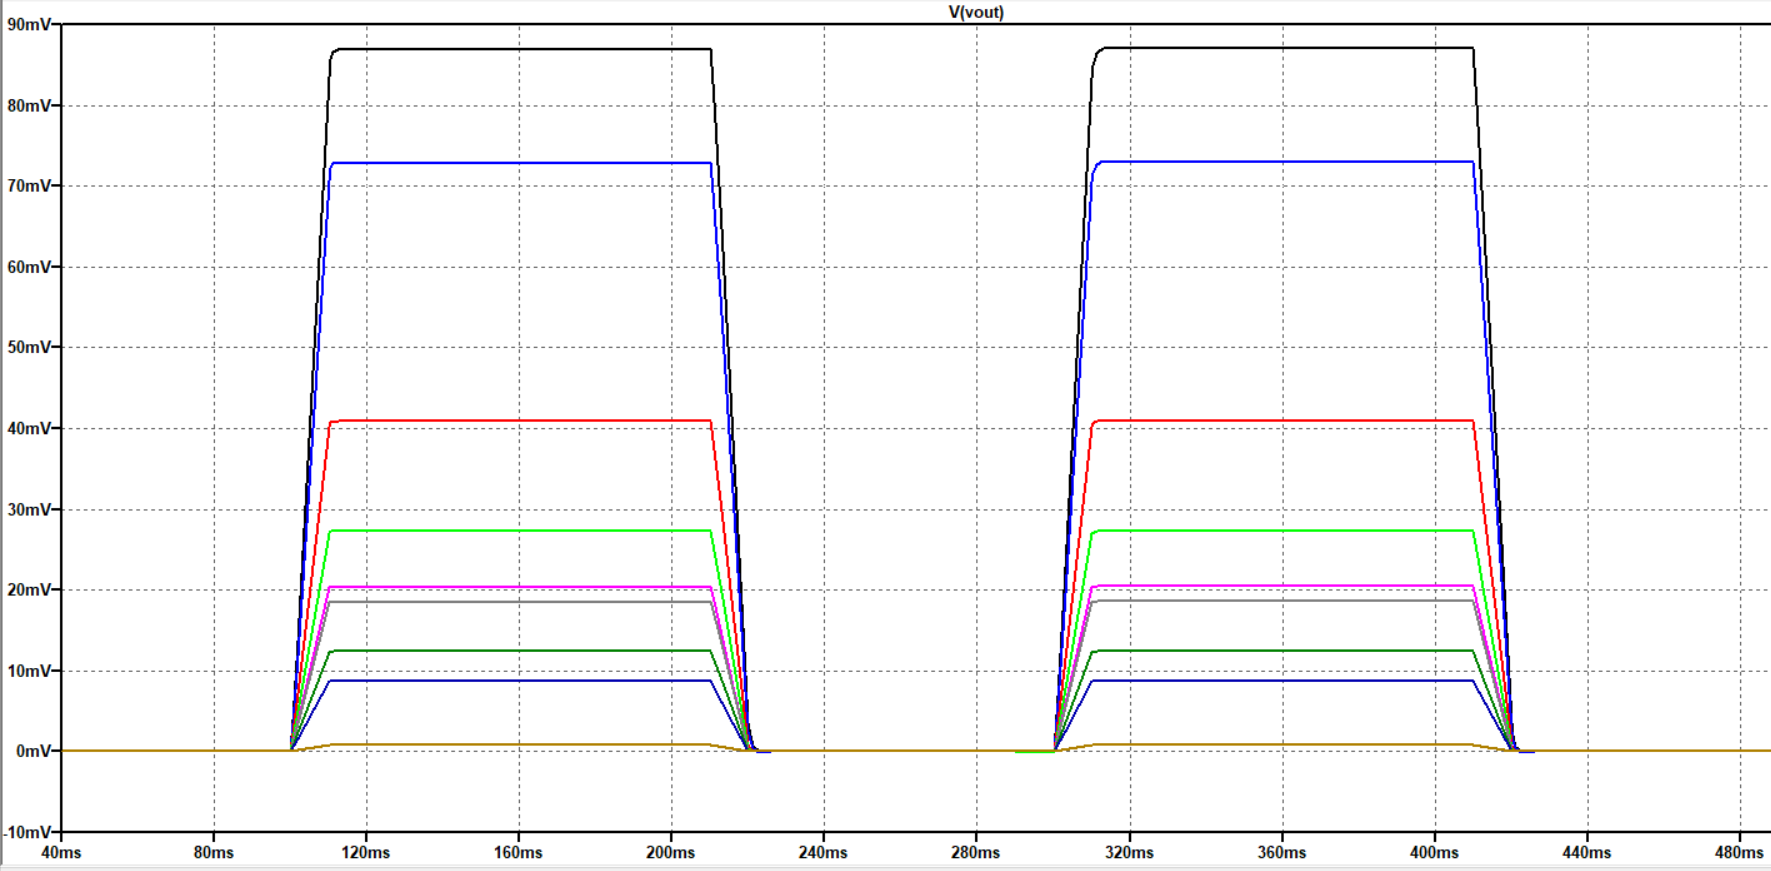
\includegraphics[width=0.5\linewidth]{ParameterSweepOP07.png}
        \caption{R2 Parameter Sweep Result}
        \label{fig:Param Sweep}
 \end{figure}

The smaller resistor values of R2 lead to a larger voltage gain and the reverse was true for large values of R2, 33k{\ohm} best matched our requirements achieving a maximum output voltage of around 12.42mV for an input voltage of $41{\mu}V$.

\end{document}
